\begin{enumerate}[label=\thesubsection.\arabic*.,ref=\thesubsection.\theenumi]
\numberwithin{equation}{enumi}

\item Find the expression of peak overshoot for a second order control system.

\solution

The transfer function for a second order control system is:
\begin{align}
    \frac{C(s)}{R(s)}= \frac{\omega_n^2}{s^2 + 2\zeta\omega_ns + \omega_n^2}
\end{align}

To calculate the unit step response,
\begin{align}
    r(t) = 1 \implies R(s) = \frac{1}{s}    
\end{align}

On Simplifying, 

\begin{align}
    C(s) = \frac{1}{s}-\frac{s+\zeta\omega_n}{(s + \zeta\omega_n)^2 + \omega_d^2} - \frac{\zeta\omega_n}{\omega_d}.\frac{\omega_d}{(s + \zeta\omega_n)^2 + \omega_d^2}  
\end{align}

where, 
\begin{align}
    \omega_d=\omega_n\sqrt{1-\zeta^2}
\end{align}

In time domain, 
\begin{align}
    c(t) = \mathcal{L}^{-1}{C(s)}
\end{align}

\begin{align}
    \implies
    c(t) = 1 - e^-\zeta\omega_nt(cos\omega_dt+\dfrac{\zeta}{\sqrt{1-\zeta^2}}.sin\omega_dt)
    \label{eq:eebtech11045_ct}
\end{align}

 \textbf{Peak Overshoot:}
Peak overshoot Mp is defined as the deviation of the response at peak time from the final value of response.
\begin{align}
    \implies M_p = c(t_p) - c(\infty)
    \label{eq:eebtech11045_Mp}
\end{align}

At $t_p$:
\begin{align}
    \frac{dc(\emph{t})}{d(\emph{t})} = 0
\end{align}

Applying this condition on \eqref{eq:eebtech11045_ct}:
\begin{align}
    \implies t_p = \frac{\pi}{\omega_n\sqrt{1-\zeta^2}}
\end{align}

Substituting $t_p$ in \eqref{eq:eebtech11045_ct}:
\begin{align}
    c(t_p) = 1 + e^{\frac{-\zeta\pi}{\sqrt{1-\zeta^2}}}
\end{align}

From \eqref{eq:eebtech11045_ct}:
\begin{align}
    \lim_{t \to \infty} c(t) = 1
\end{align}

Substituting the value of $c(t_p)$ and $c(\infty)$ in \eqref{eq:eebtech11045_Mp}:
\begin{align}
    M_p (PeakOvershoot) = e^{\frac{-\zeta\pi}{\sqrt{1-\zeta^2}}}
    \label{eq:ee18btech11045_Mp}
\end{align}

\item Find the peak Overshoot for the following second order control system
\begin{align}
    G(S) = \frac{100}{s^2 + 10s +100}
\end{align}

\solution

For the given Equation : 
\begin{align}
   \zeta = 0.5
\end{align}

Substitute this value of zeta in \eqref{eq:ee18btech11045_Mp} to get:
\begin{align}
     M_p = 0.163
\end{align}

\item Verify using a Python Plot

\solution

\begin{lstlisting}
codes/ee18btech11045.py
\end{lstlisting}

\begin{figure}[!h]
    \centering
    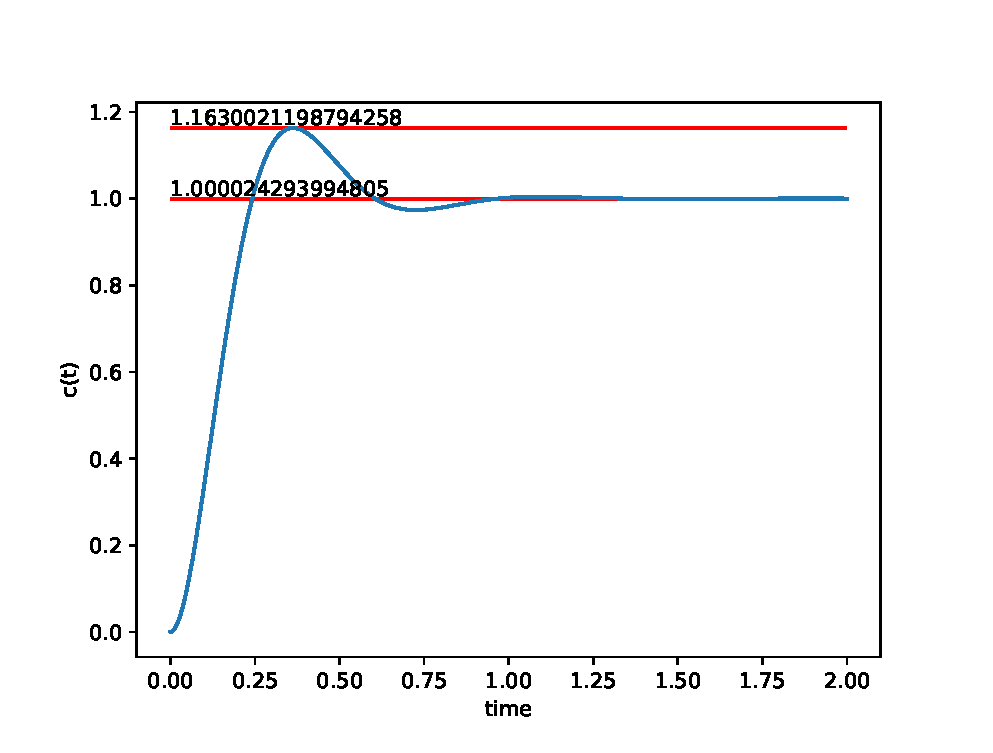
\includegraphics[width=\columnwidth]{figs/ee18btech11045/ee18btech11045.eps}
\end{figure}

\end{enumerate}